\begin{hide}
\begin{theorem}\cite{Giaro1999}
\label{t3_Giaro_14} Բոլոր երկկողմանի գրաֆները, որոնք ունեն առավելագույնը $14$ գագաթ միջակայքային ներկելի են:
\end{theorem}
\end{hide}

Փոքր առավելագույն աստիճանով երկկողմանի գրաֆների միջակայքային ներկելիության վերաբերյալ հայտնի են մի շարք արդյունքներ: Մասնավորապես, եթե $G$-ն երկկողմանի գրաֆ է, որի համար 
$\Delta(G)\leq 3$, ապա $G\in \mathfrak{N}$ և $w(G)\leq 4$\footnote{H.M. Hansen, Scheduling with minimum waiting periods, Master's Thesis, Odense University, Odense, Denmark, 1992 (դանիերեն).}: Երբ $\Delta(G) \leq 4$ և $G$-ն չունի $3$ աստիճան ունեցող գագաթ, ապա $G\in \mathfrak{N}$ և $w(G)=4$: Նաև հայտնի է, որ $G$ երկկողմանի գրաֆի համար միջակայքային $\Delta(G)$-ներկման գոյությունը կարելի է պարզել բազմանդամային ժամանակում, երբ $\Delta(G)\leq 4$, և $NP$-լրիվ է, եթե $\Delta(G)\geq 5$\footnote{K. Giaro, The complexity of consecutive $\Delta $-coloring of bipartite graphs: $4$ is easy, $5$ is hard, Ars Combin. 47, 1997, pp. 287-298.}: Միջակայքային ներկում չունեցող երկկողմանի գրաֆների օրինակներ կառուցվել են Միրումյանի, Սեվաստյանովի, Էրդյոշի, Հերցի, դե Վերրայի և Մալաֆիյսկու կողմից: Ջենսենը և Տոֆտը առաջարկել են հետևյալ խնդիրը.

\begin{hide}
\begin{theorem}
\label{t3_Hansen_Delta3}\cite{Hansen1992} Եթե $G$-ն երկկողմանի գրաֆ է, որի համար 
$\Delta(G)\leq 3$, ապա $G\in \mathfrak{N}$ և $w(G)\leq 4$.
\end{theorem}

\begin{theorem}
\label{t3_Giaro_Delta4_no3}\cite{Giaro1997}. Եթե $G$-ն երկկողմանի գրաֆ է, 
$\Delta(G)=4$ և այն չունի $3$ աստիճան ունեցող գագաթ, ապա $G\in
\mathfrak{N}$ և $w(G)=4$.
\end{theorem}

\begin{theorem}
\label{t3_Giaro_complexity}\cite{Giaro1997}. $G$ երկկողմանի գրաֆի համար միջակայքային $\Delta(G)$-ներկման գոյությունը կարելի է պարզել բազմանդամային ժամանակում, երբ $\Delta(G)\leq 4$, և $NP$-լրիվ է, եթե $\Delta(G)\geq 5$:
\end{theorem}

\begin{theorem}
\label{t3_GiaroKubaleMalafiejski_min3}\cite{GiaroKubaleMalafiejski1999} Եթե $G$-ն երկկողմանի գրաֆ է $(X,Y)$ կողմերով, իսկ $\min \{\vert X\vert, \vert Y\vert\}\leq 3$, ապա $G\in
\mathfrak{N}$:
\end{theorem}

\begin{figure}[h]
\begin{center}
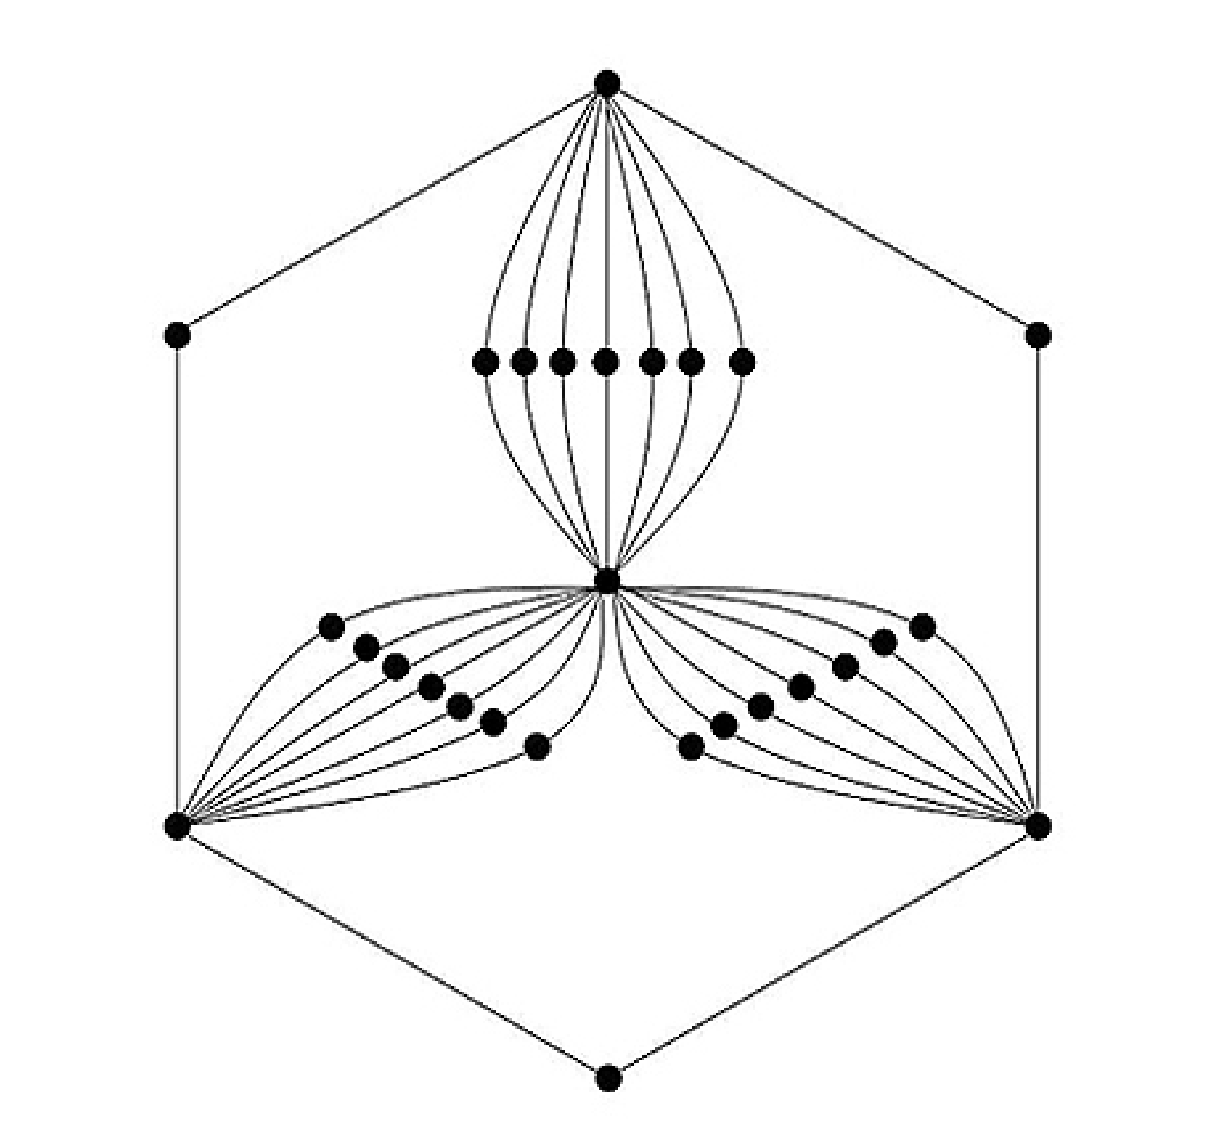
\includegraphics[width=25pc]{figures/sevastyanov.eps}\\
\caption{Սեվաստյանովի գրաֆը}\label{f3_sevastyanov}
\end{center}
\end{figure}
\end{hide}
\begin{problem}
Գոյություն ունի՞ երկկողմանի $G$ գրաֆ, որի համար $4\leq \Delta(G)\leq 12$ և
$G\notin \mathfrak{N}$:
\end{problem}

3.3 պարագրաֆում նկարագրվել են միջակայքային ներկում չունեցող երկկողմանի գրաֆների մի քանի ընտանիքներ՝ հիմնված Շեննոնի մուլտիգրաֆների, վերջավոր պրոյեկտիվ երկրաչափությունների, ծառերի և գրաֆների ենթատրոհումների վրա:

\begin{hide}
\begin{theorem}
\label{t3_Shannon} Եթե $r\geq 5$, ապա $\Delta_{r,s,t}\notin
\mathfrak{N}$:
\end{theorem}
\begin{proof}[Ապացույց]
Ենթադրենք հակառակը՝ $\Delta_{r,s,t}$ գրաֆը ունի  $\alpha$ միջակայքային $q$-ներկում ինչ որ $q$-ի համար, $q\geq r+s+t$:

Դիտարկենք $v$ գագաթը: Ենթադրենք $u$-ն և $w$-ն $v$-ին հարևան այն գագաթներն են, որոնց համար $\alpha(vu)=\underline{S}(v,\alpha)=p$ և
$\alpha(vw)=\overline{S}(v,\alpha)=p+r+s+t-1$: 
$\Delta_{r,s,t}$-ի կառուցման համաձայն $\Delta_{r,s,t}-v$ գրաֆում գոյություն ունի երկու երկարությամբ $P(u,w)$ շղթա, որը միացնում է $u$-ն  $w$-ին, որտեղ
\begin{center}
$P(u,w)=(u,uv^{\prime},v^{\prime},v^{\prime}w,w)$:
\end{center}

Քանի որ $d(u)=3$ և $d(v^{\prime})\leq s+t$, ունենք, որ

\begin{center}
$\alpha(uv^{\prime})\leq p+d(u)-1=p+2$, ուստի
\end{center}
\begin{center}
$\alpha(v^{\prime}w)\leq p+2+ d(v^{\prime})-1=p+1+s+t$:
\end{center}

Մյուս կողմից, քանի որ $d(w)=3$, ունենք, որ

\begin{center}
$p+r+s+t-1=\alpha(vw)=\overline{S}(v,\alpha)\leq p+1+s+t+d(w)-1=p+s+t+3$:
\end{center}
Այսպիսով, ստացանք, որ $r\leq 4$, ինչը հակասություն է:
\end{proof}

\begin{figure}[h]
\begin{center}
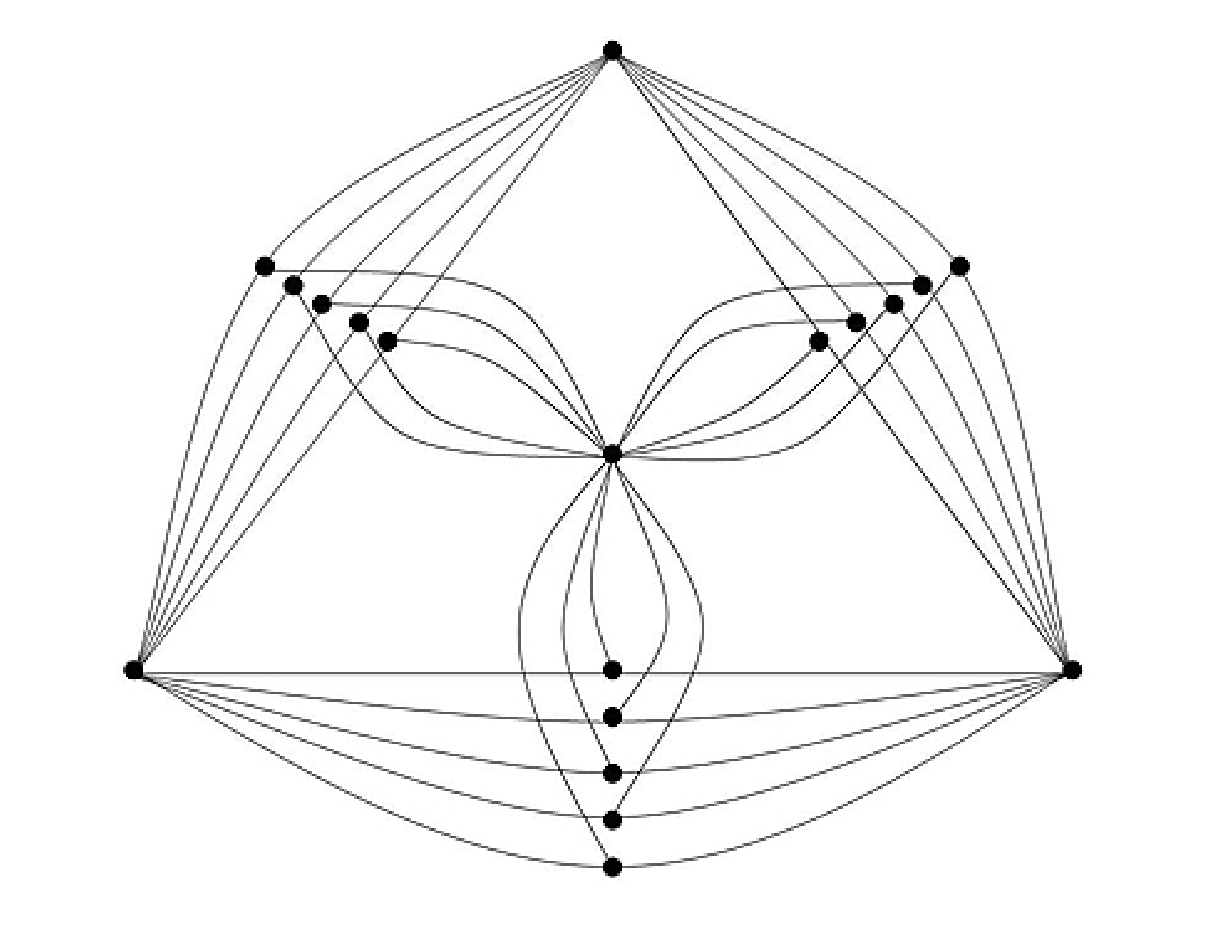
\includegraphics[width=30pc]{figures/shannon555.eps}\\
\caption{$\Delta_{5,5,5}$ գրաֆը}\label{f3_Shannon555}
\end{center}
\end{figure}

\begin{corollary}
\label{c3_Shannon} Ցանկացած $\Delta$ բնական թվի համար, $\Delta \geq 15$,
գոյություն ունի կապակցված երկկողմանի գրաֆ $G$, այնպես, որ $G\notin \mathfrak{N}$
և $\Delta(G)=\Delta$:
\end{corollary}

\begin{figure}[t]
\begin{center}
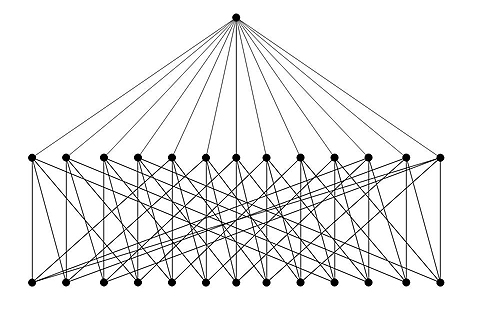
\includegraphics[width=30pc]{figures/erd13.jpg}\\
\caption{$Erd(1,1,1,1,1,1,1,1,1,1,1,1,1)$ գրաֆը:}\label{f3_Erd}
\end{center}
\end{figure}

\begin{theorem}
\label{t3_Erdos} Եթե $\underset{i=n+2}{\overset{n^{2}+n+1}{\sum
}}r_{i}> 2(n+1)$, ապա $Erd(r_{1},\ldots,r_{n^{2}+n+1})\notin
\mathfrak{N}$.
\end{theorem}
\begin{proof}[Ապացույց]
Ենթադրենք հակառակը.
$Erd(r_{1},\ldots,r_{n^{2}+n+1})$ գրաֆը ունի $\alpha$ միջակայքային $t$-ներկում
ինչ որ $t$-ի համար, $t\geq \underset{i=1}{\overset{n^{2}+n+1}{\sum
}}r_{i}$:

Դիտարկենք $u$ գագաթը: Դիցուք $v_{p}^{(l_{i_{0}})}$-ն և
$v_{q}^{(l_{j_{0}})}$-ն $u$-ին հարևան այն գագաթներն են, որոնց համար 
$\alpha\left(uv_{p}^{(l_{i_{0}})}\right)=\underline{S}(u,\alpha)=s$ և
$\alpha\left(uv_{q}^{(l_{j_{0}})}\right)=\overline{S}(u,\alpha)=s+\underset{i=1}{\overset{n^{2}+n+1}{\sum
}}r_{i}-1$:

Եթե $l_{i_{0}}=l_{j_{0}}$, ապա, ըստ 
$Erd(r_{1},\ldots,r_{n^{2}+n+1})$-ի կառուցման, գոյություն ունի $k_{0}$ այնպիսին, որ
$k_{0}v_{p}^{(l_{i_{0}})}$, $k_{0}v_{q}^{(l_{j_{0}})}\in
E(Erd(r_{1},\ldots,r_{n^{2}+n+1}))$: Եթե $l_{i_{0}}\neq l_{j_{0}}$,
ապա, ըստ $Erd(r_{1},\ldots,r_{n^{2}+n+1})$-ի կառուցման և
Հ2 հատկության, գոյություն ունի $k_{0}$ այնպիսին, որ
$k_{0}v_{p}^{(l_{i_{0}})}$, $k_{0}v_{q}^{(l_{j_{0}})}\in
E(Erd(r_{1},\ldots,r_{n^{2}+n+1}))$:

$Erd(r_{1},\ldots,r_{n^{2}+n+1})$-ի կառուցման համաձայն, ինչպես նաև Հ3 և Հ4 հատկություններից ելնելով ունենք, որ
$d\left(v_{p}^{(l_{i_{0}})}\right)=d\left(v_{q}^{(l_{j_{0}})}\right)=n+2$
և
\begin{center}
$\alpha\left(k_{0}v_{p}^{(l_{i_{0}})}\right)\leq
s+d\left(v_{p}^{(l_{i_{0}})}\right)-1=s+n+1$, ուստի
\end{center}
\begin{center}
$\alpha\left(k_{0}v_{q}^{(l_{j_{0}})}\right)\leq
s+n+1+d(k_{0})-1\leq s+n+\underset{i=1}{\overset{n+1}{\sum }}r_{i}$:
\end{center}

Հետևաբար,
\begin{center}
$s+\underset{i=1}{\overset{n^{2}+n+1}{\sum
}}r_{i}-1=\alpha\left(uv_{q}^{(l_{j_{0}})}\right)=\overline{S}(u,\alpha)\leq
s+n+\underset{i=1}{\overset{n+1}{\sum
}}r_{i}+d\left(v_{q}^{(l_{j_{0}})}\right)-1=s+2n+1+\underset{i=1}{\overset{n+1}{\sum
}}r_{i}$:
\end{center}

Այսպիսով ստանում ենք, որ $\underset{i=n+2}{\overset{n^{2}+n+1}{\sum }}r_{i}\leq
2(n+1)$, ինչը հակասություն է:
\end{proof}

\begin{corollary}
\label{c3_Erdos} Ցանկացած բնական $\Delta$-ի համար, $\Delta \geq 13$,
գոյություն ունի կապակցված երկկողմանի գրաֆ $G$, այնպես, որ $G\notin \mathfrak{N}$
և $\Delta(G)=\Delta$:
\end{corollary}

\begin{figure}[h]
\begin{center}
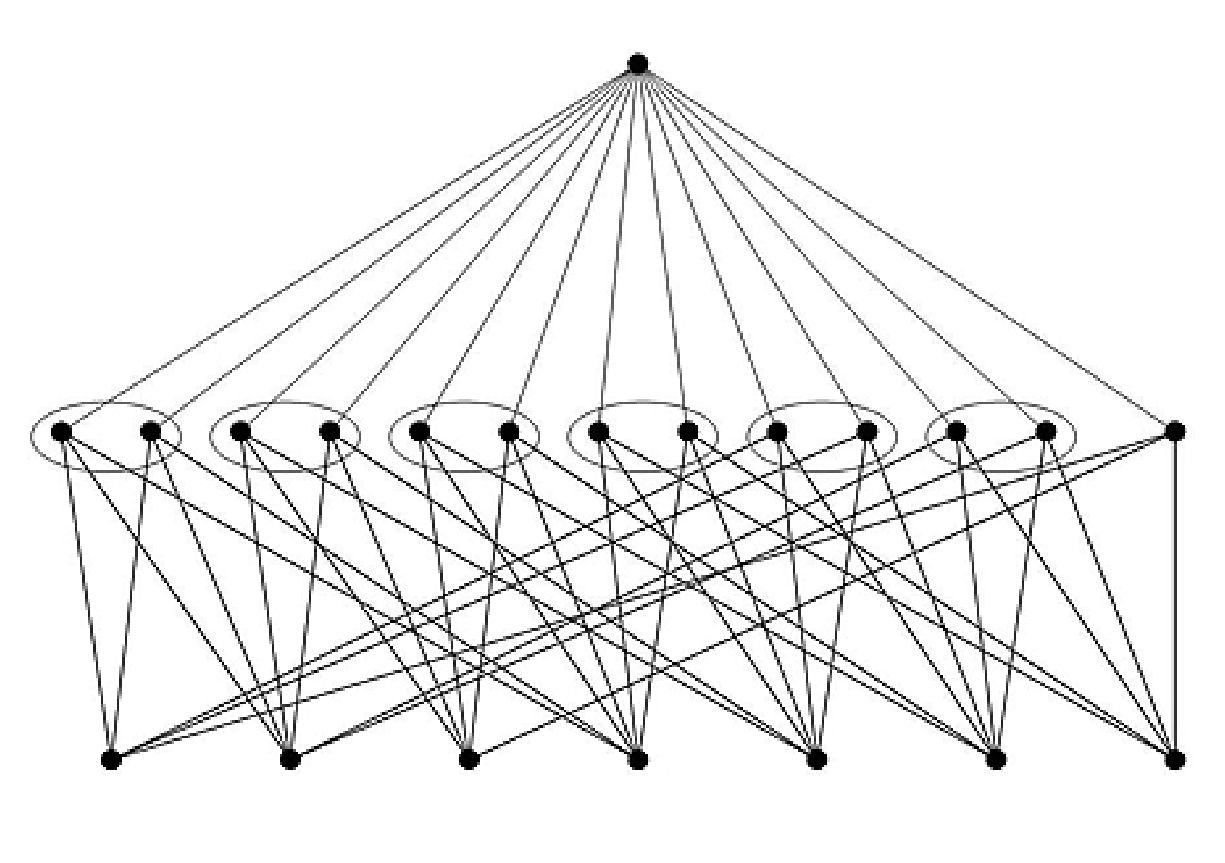
\includegraphics[width=30pc]{figures/erd6x2_1.eps}\\
\caption{$Erd(2,2,2,2,2,2,1)$ գրաֆը:}\label{f3_Erd6x2_1}
\end{center}
\end{figure}
\begin{theorem}
\label{t3_Kamalian_tree} Եթե $T$-ն ծառ է, ապա $T$-ն ունի միջակայքային $t$-ներկում այն և միայն այն դեպքում $\Delta(T)\leq t\leq M(T)$:
\end{theorem}

\begin{theorem}
\label{t3_tree} Եթե $T$-ն ծառ է, իսկ $\vert F(T)\vert >
M(T)+2$, ապա $\widetilde{T}\notin \mathfrak{N}$:
\end{theorem}
\begin{proof}[Ապացույց]
Ենթադրենք հակառակը, $\widetilde{T}$-ն ունի $\alpha$ միջակայքային $t$-ներկում ինչ որ $t$-ի համար, $t\geq \vert F(T)\vert$:

Դիտարկենք $u$ գագաթը: Դիցուք $v$-ն և $v^{\prime}$-ը $u$-ի հարևան այն երկու գագաթներն են, որոնց համար $\alpha(uv)=\underline{S}(u,\alpha)=s$ և
$\alpha(uv^{\prime})=\overline{S}(u,\alpha)=s+\vert F(T)\vert-1$: Քանտի որ $\widetilde{T}-u$ գրաֆը ծառ է, այնտեղ գոյություն ունի միակ շղթա
$P(v,v^{\prime})$, որը միացնում է $v$-ն և $v^{\prime}$-ը, որտեղ
\begin{center}
$P(v,v^{\prime})=(x_{1},e_{1},x_{2},\ldots,x_{i},e_{i},x_{i+1},\ldots,x_{k},e_{k},x_{k+1})$,
$x_{1}=v$, $x_{k+1}=v^{\prime}$:
\end{center}

Նկատենք, որ.
\begin{center}
$\alpha(x_{i}x_{i+1})\leq s+1+\underset{j=1}{\overset{i}{\sum
}}(d_{T}(x_{j})-1)$, երբ $1\leq i\leq k$:
\end{center}

Ստանում ենք, որ
\begin{center}
$\alpha(x_{k}x_{k+1})=\alpha(x_{k}v^{\prime})\leq
s+1+\underset{j=1}{\overset{k}{\sum
}}(d_{T}(x_{j})-1)=s+LP(v,v^{\prime})\leq s+M(T)$:
\end{center}

Այսպիսով,
\begin{center}
$s+\vert F(T)\vert -1=\overline{S}(u,\alpha)=\alpha(uv^{\prime})\leq
s+1+M(T)$, ուստի $\vert F(T)\vert\leq M(T)+2$,
\end{center}
ինչը հակասություն է:
\end{proof}

\begin{corollary}
\label{c3_tree} Եթե $T$-ն այնպիսի ծառ է, որի ցանկացած երկու կախված գագաթների միջև հեռավորությունը զույգ է և $\vert F(T)\vert >
M(T)+2$, ապա $\widetilde{T}$ երկկողմանի գրաֆը չունի միջակայքային ներկում:
\end{corollary}

\begin{figure}[h]
\begin{center}
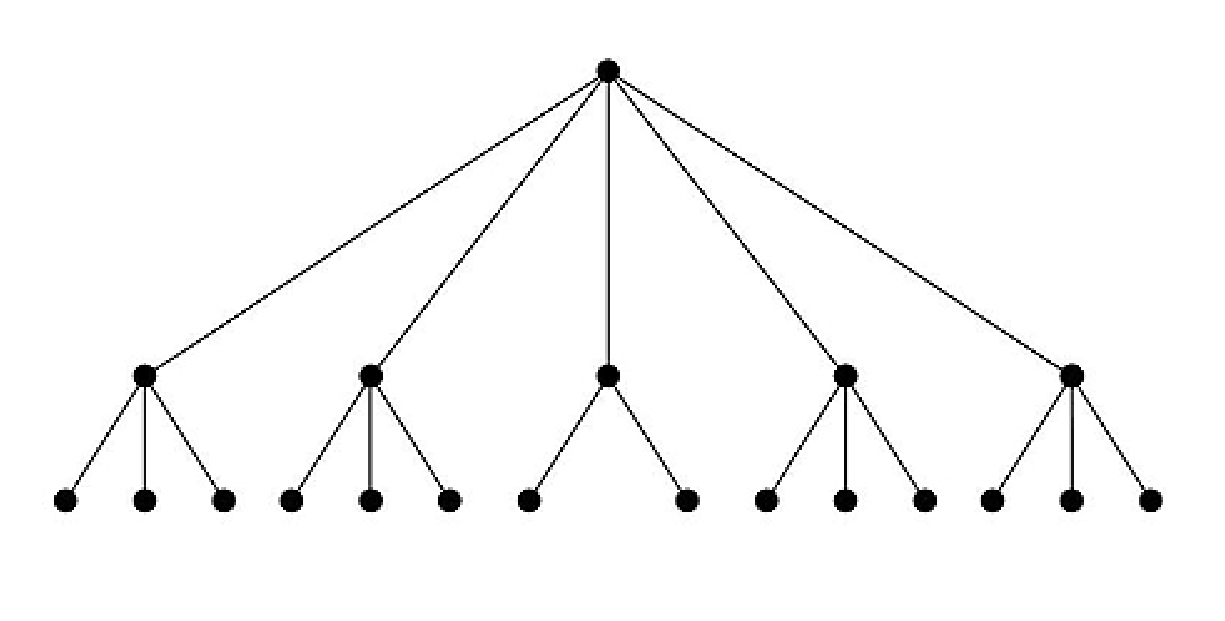
\includegraphics[width=20pc]{figures/tree.eps}\\
\caption{$T$ ծառը}\label{f3_tree}
\end{center}
\end{figure}
\end{hide}

Դիցուք $G$-ն գրաֆ է, $V(G)=\{v_{1},\ldots,v_{n}\}$: Սահմանենք 
$S(G)$ և $\widehat{G}$ գրաֆները հետևյալ կերպ.
\begin{align*}
V(S(G))&=\{v_{1},\ldots,v_{n}\}\cup \{w_{ij}:v_{i}v_{j}\in E(G)\},\\
E(S(G))&=\{v_{i}w_{ij},v_{j}w_{ij}:v_{i}v_{j}\in E(G)\},\\
V(\widehat{G})&=V(S(G))\cup \{u\}\text{, որտեղ } u\notin V(S(G)),\\
E(\widehat{G})&=E(S(G))\cup \{uw_{ij}:v_{i}v_{j}\in E(G)\}:
\end{align*}
$S(G)$ գրաֆը կոչվում է $G$-ի ենթատրոհում:

\begin{remark}
\label{r3_S(G)} Եթե $G$-ն երկկողմանի գրաֆ է և $G\in
\mathfrak{N}$, ապա $S(G)\in \mathfrak{N}$:
\end{remark}
\begin{proof}[Ապացույց]
Դիցուք $G$-ն երկկողմանի գրաֆ է $(X,Y)$ մասերով, որտեղ
$X=\{x_{1},\ldots,x_{r}\}$, $Y=\{y_{1},\ldots,y_{s}\}$, իսկ 
$\alpha$-ն $G$-ի միջակայքային $t$-ներկում է:

Սահմանենք $S(G)$-ի $\beta$ միջակայքային ներկումը հետևյալ կերպ.
\begin{center}
$\beta(x_{i}w_{ij})=\alpha(x_{i}y_{j})$ և
$\beta(y_{j}w_{ij})=\alpha(x_{i}y_{j})+1$, ցանկացած $x_{i}y_{j}\in
E(G)$-ի համար:
\end{center}

Հեշտ է համոզվել, որ $\beta$-ն $S(G)$-ի միջակայքային $(t+1)$-ներկում է:
\end{proof}

Հայտնի է\footnote{D. Hanson, C.O.M. Loten, B. Toft, On interval colorings of bi-regular bipartite graphs, Ars Combin. 50, 1998, pp. 23-32.}\textsuperscript{,}\footnote{Р.Р. Камалян, А.Н. Мирумян, Интервальные реберные раскраски двудольных графов одного класса, Доклады НАН РА, том 97, N 4, 1997, стр. 3-5.}, որ եթե $G$-ն համասեռ գրաֆ է, ապա $S(G)\in \mathfrak{N}$: Պետրոսյանը և Խաչատրյանը 2011-ին առաջարկել էին հիպոթեզ, համաձայն որի, եթե $G\in \mathfrak{N}$, ապա $S(G)\in \mathfrak{N}$: Այս հիպոթեզը հաստատվել է Պյատկինի կողմից\footnote{А.В. Пяткин, Об интервальной (1,1)-раскраске инциденторов интервально раскрашиваемых графов, Дискретн. анализ и исслед. опер. 22:2, 2015, стр. 63-72.}:
\begin{hide}
\begin{hypothesis}
Եթե $G\in \mathfrak{N}$, ապա $S(G)\in \mathfrak{N}$:
\end{hypothesis}
\end{hide}
\begin{theorem}
\label{t3_subdivision_paths} Եթե $G$-ն կապացված գրաֆ է, և
\begin{center}
$\vert E(G)\vert
> 1+ {\max\limits_{P\in \mathbf{P}}}{\sum\limits_{v\in
V(P)}}\ \left(d_{\widehat{G}}(v)-1\right)$,
\end{center}
որտեղ $\mathbf{P}$-ն $S(G)$-ում $w_{ij}$ գագաթները միացնող ամենակարճ շղթաների բազմությունն է, ապա $\widehat{G}\notin \mathfrak{N}$:
\end{theorem}
\begin{proof}[Ապացույց]
Ենթադրենք հակառակը, $\alpha$-ն $\widehat{G}$-ի միջակայքային 
$t$-ներկում է ինչ որ $t$-ի համար, $t\geq \vert E(G)\vert$:

Դիտարկենք $u$ գագաթը: Դիցուք $w$-ն և $w^{\prime}$-ը $u$-ին հարևան այն երկու գագաթներն են, որոնց համար $\alpha(uw)=\underline{S}(u,\alpha)=s$ և
$\alpha(uw^{\prime})=\overline{S}(u,\alpha)=s+\vert E(G)\vert-1$: Քանի որ $\widehat{G}-u=S(G)$ և $\widehat{G}-u$ գրաֆները կապակցված են, գոյություն ունի $w$-ն և $w^{\prime}$-ը միացնող կարճագույն $P(w,w^{\prime})$ շղթա $\widehat{G}-u$ գրաֆում, որտեղ
\begin{center}
$P(w,w^{\prime})=(x_{1},e_{1},x_{2},\ldots,x_{i},e_{i},x_{i+1},\ldots,x_{k},e_{k},x_{k+1})$,
$x_{1}=w$, $x_{k+1}=w^{\prime}$:
\end{center}

Նկատենք, որ
\begin{center}
$\alpha(x_{i}x_{i+1})\leq s+\underset{j=1}{\overset{i}{\sum
}}(d_{\widehat{G}}(x_{j})-1)$, երբ $1\leq i\leq k$
\end{center}
և
\begin{center}
$\alpha(x_{k+1}u)=\alpha(w^{\prime}u)\leq
s+\underset{j=1}{\overset{k+1}{\sum }}(d_{\widehat{G}}(x_{j})-1)$:
\end{center}

Հետևաբար,
\begin{center}
$s+\vert E(G)\vert -1=\overline{S}(u,\alpha)=\alpha(uw^{\prime})\leq
s+\underset{j=1}{\overset{k+1}{\sum }}(d_{\widehat{G}}(x_{j})-1)\leq
s+{\max\limits_{P\in \mathbf{P}}}{\sum\limits_{v\in V(P)}}\
\left(d_{\widehat{G}}(v)-1\right)$,
\end{center}
ուստի՝
\begin{center}
$\vert E(G)\vert \leq 1+{\max\limits_{P\in
\mathbf{P}}}{\sum\limits_{v\in V(P)}}\
\left(d_{\widehat{G}}(v)-1\right)$,
\end{center}
ինչը հակասություն է:
\end{proof}

\begin{hide}
\begin{corollary}
\label{c3_subdivision_complete} Եթե $n\geq 7$, ապա $\widehat{K}_{n}\notin
\mathfrak{N}$:
\end{corollary}
\begin{corollary}
\label{c3_subdivision_complete_bipartite} Եթե $mn-m-n>5$, ապա $\widehat{K}_{m,n}\notin \mathfrak{N}$:
\end{corollary}

\begin{figure}[h]
\begin{center}
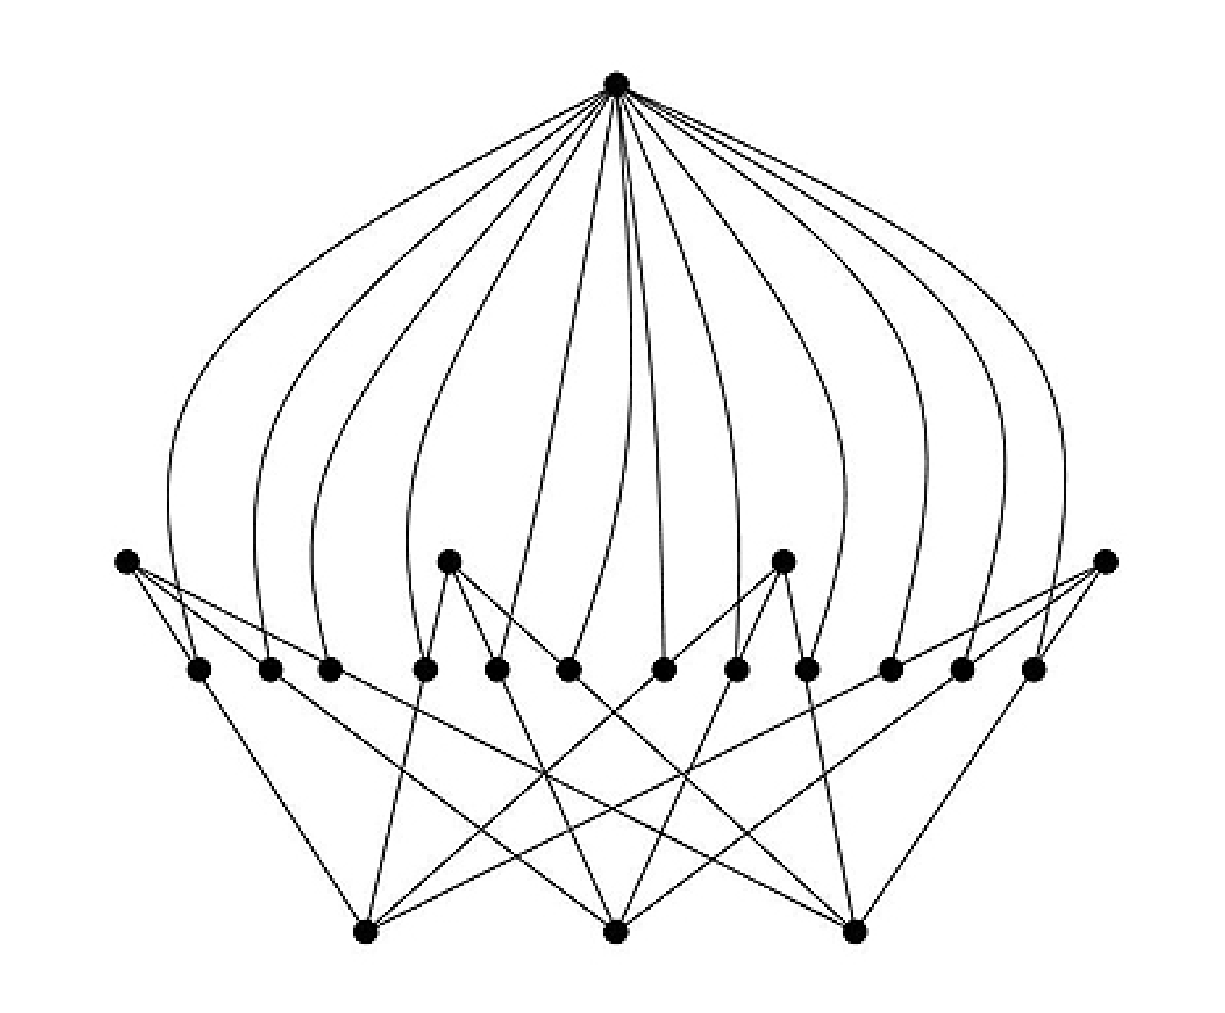
\includegraphics[width=25pc]{figures/subdivisionK34.eps}\\
\caption{$\widehat{K}_{3,4}$ գրաֆը:}\label{f3_subdivisionK34}
\end{center}
\end{figure}


\begin{theorem}
\label{t3_subdivision_K34} $\widehat{K}_{3,4}\notin \mathfrak{N}$:
\end{theorem}
\begin{proof}[Ապացույց]
Դիցուք
$V(\widehat{K}_{3,4})=\{u,v_{1},v_{2},v_{3},v_{4},v_{5},v_{6},v_{7}\}\cup
\{w_{ij}:1\leq i\leq 3, 4\leq j\leq 7\}$, իսկ
$E(\widehat{K}_{3,4})=\{v_{i}w_{ij},v_{j}w_{ij},uw_{ij}:1\leq i\leq
3, 4\leq j\leq 7\}$:

Ենթադրենք, որ $\alpha$-ն $\widehat{K}_{3,4}$-ի միջակայքային $t$-ներկում է ինչ որ $t$-ի համար, $t\geq 12$:

Դիտարկենք $u$ գագաթը: Դիցուք $w_{i_{0}j_{0}}$-ն և $w_{i_{1}j_{1}}$-ն
$u$-ին հարևան այն գագաթներն են, որոնց համար 
$\alpha(uw_{i_{0}j_{0}})=\underline{S}(u,\alpha)=s$ և
$\alpha(uw_{i_{1}j_{1}})=\overline{S}(u,\alpha)=s+11$: Դիտարկենք երկու դեպք:

Դեպք 1. $i_{0}=i_{1}$ կամ $j_{0}=j_{1}$:

Եթե $i_{0}=i_{1}$, ապա
$v_{i_{0}}w_{i_{0}j_{0}},v_{i_{0}}w_{i_{0}j_{1}}\in
E(\widehat{K}_{3,4})$: Հետևաբար,

\begin{center}
$\alpha(v_{i_{0}}w_{i_{0}j_{0}})\leq s+2$ և
$\alpha(v_{i_{0}}w_{i_{0}j_{1}})\leq s+5$:
\end{center}

Ուստի,
\begin{center}
$s+11=\overline{S}(u,\alpha)=\alpha(uw_{i_{0}j_{1}})\leq s+7$,
\end{center}
ինչը հնարավոր չէ:

Եթե $j_{0}=j_{1}$, ապա
$v_{j_{0}}w_{i_{0}j_{0}},v_{j_{0}}w_{i_{1}j_{0}}\in
E(\widehat{K}_{3,4})$: Հետևաբար,

\begin{center}
$\alpha(v_{j_{0}}w_{i_{0}j_{0}})\leq s+2$ և
$\alpha(v_{j_{0}}w_{i_{1}j_{0}})\leq s+4$:
\end{center}

Ուստի,
\begin{center}
$s+11=\overline{S}(u,\alpha)=\alpha(uw_{i_{1}j_{0}})\leq s+6$,
\end{center}
ինչը նույնպես հնարավոր չէ:

Դեպք 2. $i_{0}\neq i_{1}$ և $j_{0}\neq j_{1}$:

Այս դեպքում $v_{i_{0}}v_{j_{0}}$ և $v_{i_{1}}v_{j_{1}}$ կողերը անկախ են $K_{3,4}$-ում: Իսկ
$K_{3,4}$-ում ցանկացած երկու անկախ կող ընկած են 4 երկարությամբ ցիկլի վրա: Այսինքն, $\widehat{K}_{3,4}$-ում գոյություն ունի ցիկլ
$C=w_{i_{0}j_{0}}v_{j_{0}}w_{i_{1}j_{0}}v_{i_{1}}w_{i_{1}j_{1}}v_{j_{1}}w_{i_{0}j_{1}}v_{i_{0}}w_{i_{0}j_{0}}$, որը բաղկացած է $P$ և $Q$ շղթաներից, որտեղ
\begin{center}
$P=\left(w_{i_{0}j_{0}},v_{j_{0}}w_{i_{0}j_{0}},v_{j_{0}},v_{j_{0}}w_{i_{1}j_{0}},w_{i_{1}j_{0}},v_{i_{1}}w_{i_{1}j_{0}},v_{i_{1}},v_{i_{1}}w_{i_{1}j_{1}},w_{i_{1}j_{1}}\right)$
\end{center}
և
\begin{center}
$Q=\left(w_{i_{0}j_{0}},v_{i_{0}}w_{i_{0}j_{0}},v_{i_{0}},v_{i_{0}}w_{i_{0}j_{1}},w_{i_{0}j_{1}},v_{j_{1}}w_{i_{0}j_{1}},v_{j_{1}},v_{j_{1}}w_{i_{1}j_{1}},w_{i_{1}j_{1}}\right)$:
\end{center}

Եթե $\alpha(v_{j_{0}}w_{i_{0}j_{0}})\leq s+1$, ապա դիտարկելով $P$ շղթան ստանում ենք, որ $\alpha(v_{i_{1}}w_{i_{1}j_{1}})\leq s+8$ և
$\overline{S}(w_{i_{1}j_{1}},\alpha)\leq s+10$, ինչը հակասություն է:

Եթե $\alpha(v_{i_{0}}w_{i_{0}j_{0}})\leq s+1$, ապա դիտարկելով $Q$ շղթան ստանում ենք, որ $\alpha(v_{j_{1}}w_{i_{1}j_{1}})\leq s+8$ և
$\overline{S}(w_{i_{1}j_{1}},\alpha)\leq s+10$, ինչը ևս հակասություն է:

Ուստի, $\alpha(v_{j_{0}}w_{i_{0}j_{0}})\geq s+2$ և
$\alpha(v_{i_{0}}w_{i_{0}j_{0}})\geq s+2$, ինչը կրկին հակասություն է:
\end{proof}


\begin{figure}[h]
\begin{center}
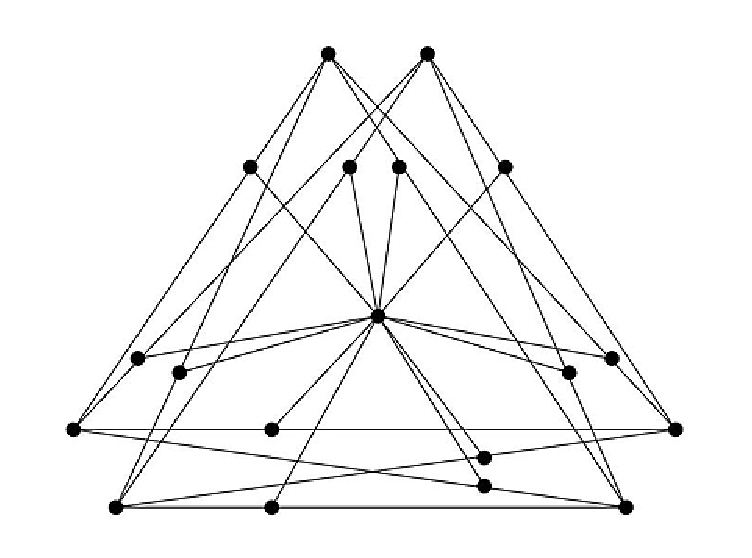
\includegraphics[width=25pc]{figures/K222.eps}\\
\caption{$\widehat{K}_{2,2,2}$ գրաֆը:}\label{f3_K222}
\end{center}
\end{figure}

\begin{theorem}
\label{t3_subdivision_K222} $\widehat{K}_{2,2,2}\notin \mathfrak{N}$:
\end{theorem}
\begin{proof}[Ապացույց]
Դիցուք
\begin{align*}
V(\widehat{K}_{2,2,2}) &=\{u,v_{1},v_{2},v_{3},v_{4},v_{5},v_{6}\}\cup
\{w_{ij}:1\leq i<j\leq 6,(i,j)\notin \{(1,2),(3,4),(5,6)\}\}\\
E(\widehat{K}_{2,2,2}) &=\{v_{i}w_{ij},v_{j}w_{ij},uw_{ij}:1\leq
i<j\leq 6,(i,j)\notin \{(1,2),(3,4),(5,6)\}\}
\end{align*}
Ենթադրենք $\alpha$-ն $\widehat{K}_{2,2,2}$-ի միջակայքային $t$-ներկում է ինչ որ $t$-ի համար, $t\geq 12$:

Դիտարենք $u$ գագաթը: Դիցուք, $w_{i_{0}j_{0}}$-ն և $w_{i_{1}j_{1}}$-ը $u$-ին հարևան այն երկու գագաթներն են, որոնց համար
$\alpha(uw_{i_{0}j_{0}})=\underline{S}(u,\alpha)=s$ և
$\alpha(uw_{i_{1}j_{1}})=\overline{S}(u,\alpha)=s+11$: $\widehat{K}_{2,2,2}$ գրաֆի սիմետրիայի համաձայն կարող ենք ենթադրել, որ 
$(i_{0},j_{0})=(1,6)$: Դիտարկենք երկու դեպք:

Դեպք 1. $v_{1}v_{6}$ և $v_{i_{1}}v_{j_{1}}$ հարևան են 
$K_{2,2,2}$-ում:

$\widehat{K}_{2,2,2}$ գրաֆի սիմետրիայից ելնելով բավական է դիտարկել այն դեպքը, երբ $(i_{1},j_{1})=(1,4)$ և $(i_{1},j_{1})=(1,5)$:

Եթե $\alpha(uw_{14})=s+11$ կամ $\alpha(uw_{15})=s+11$, ապա
$\alpha(v_{1}w_{16})\leq s+2$ և $\alpha(v_{1}w_{1j_{1}})\leq s+5$:
Ուստի, $\alpha(uw_{1j_{1}})\leq s+7$, ինչը հնարավոր չէ:

Դեպք 2. $v_{1}v_{6}$ և $v_{i_{1}}v_{j_{1}}$ անկախ են $K_{2,2,2}$-ում:

Հաշվի առնելով $\widehat{K}_{2,2,2}$ գրաֆի սիմետրիան, բավական է դիտարկել այն դեպքը, երբ $(i_{1},j_{1})=(4,5)$ և $(i_{1},j_{1})=(2,5)$:

Եթե $\alpha(uw_{45})=s+11$, ապա կամ $\alpha(v_{1}w_{16})=s+1$ կամ
$\alpha(v_{1}w_{16})=s+2$, և երկու դեպքերում էլ 
$C=w_{16}v_{1}w_{15}v_{5}w_{45}v_{4}w_{46}v_{6}w_{16}$ ցիկլի վրա գտնվող կողերի գույները որոշվում են միարժեքորեն:
Հետևաբար, $\alpha(v_{1}w_{14})\leq s+4$ և
$\alpha(v_{4}w_{14})\geq s+7$, ինչը հակասություն է:

Եթե $\alpha(uw_{25})=s+11$, ապա հաշվի առնելով 
$\widehat{K}_{2,2,2}$ գրաֆի սիմետրիան կարող ենք համարել, որ $\alpha(v_{1}w_{16})=s+1$:
Այս դեպքում 
$C=w_{16}v_{1}w_{15}v_{5}w_{25}v_{2}w_{26}v_{6}w_{16}$ ցիկլի վրա գտնվող բոլոր կողերի գույները որոշվում են միարժեքորեն: Հետևաբար, $\alpha(uw_{26})=s+6$: $\widehat{K}_{2,2,2}$ գրաֆի սիմետրիան հաշվի առնելով կարող ենք համարել, որ 
$\alpha(v_{1}w_{13})=s+2$ և $\alpha(v_{1}w_{14})=s+3$: Այժմ ցույց տանք, որ $\alpha(uw_{13})=s+1$: Քանի որ $S(u,\alpha)=[s,s+11]$, պետք է գոյություն ունենա կող $uw_{i^{\prime}j^{\prime}}$ որի համար
$\alpha\left(uw_{i^{\prime}j^{\prime}}\right)=s+1$: Քանի որ
$\alpha(v_{2}w_{25})=s+10$, ստանում ենք, որ $i^{\prime},j^{\prime}
\neq 2,5$: Եթե $\left(i^{\prime},j^{\prime}\right)\in
\{(1,4),(4,6)\}$, ապա $\alpha(uw_{24})=s+6$, ինչը հնարավոր չէ, քանի որ $\alpha(uw_{26})=s+6$: Մյուս կողմից, եթե 
$\left(i^{\prime},j^{\prime}\right)=(3,6)$, ապա հաշվի առնելով, որ
$\alpha(v_{6}w_{36})>s+2$, ստանում ենք, որ $\alpha(uw_{23})=s+6$, ինչը նույնպես հնարավոր չէ, քանի որ $\alpha(uw_{26})=s+6$: Ուստի, ստանում ենք, որ
$\left(i^{\prime},j^{\prime}\right)=(1,3)$: Հետևաբար,
$\alpha(v_{3}w_{13})=s+3$ և հաշվի առնելով, որ 
$\alpha(v_{2}w_{25})=s+10$, ստանում ենք, որ $\alpha(v_{3}w_{23})=s+6$: Սրանից հետևում է, որ $\alpha(v_{3}w_{35})\leq s+5$: Մյուս կողմից, քանի որ 
$\alpha(v_{5}w_{25})=s+9$, ունենք, որ $\alpha(v_{5}w_{35})\geq s+7$, ուտսի $\alpha(uw_{35})=s+6=\alpha(uw_{26})$, ինչը հակասություն է:
\end{proof}
\end{hide}

3.3 պարագրաֆում կառուցվել են երեք գրաֆներ, որոնք մասնակիորեն պատասխանում են Ջենսենի և Տոֆտի խնդրին. $\widehat{K}_{3,4} \notin \mathfrak{N}$, որտեղ $\Delta(\widehat{K}_{3,4})=12$, $|V(\widehat{K}_{3,4})|=20$, $\widehat{K}_{2,2,2} \notin \mathfrak{N}$, որտեղ $\Delta(\widehat{K}_{2,2,2})=12$, $|V(\widehat{K}_{2,2,2})|=19$, և  $\widehat{K}_{3,4}^{\prime} \notin \mathfrak{N}$, որտեղ $\widehat{K}_{3,4}^{\prime}$ գրաֆը ստացվում է $\widehat{K}_{3,4}$ գրաֆից՝ առավելագույն աստիճան ունեցող գագաթին կից կողերից մեկը հեռացնելով ($\Delta(\widehat{K}_{3,4}^{\prime})=11$, $|V(\widehat{K}_{3,4}^{\prime})|=20$):

\begin{hide}
\begin{theorem}
\label{t3_subdivision_K34_prime} $\widehat{K}_{3,4}^{\prime}\notin
\mathfrak{N}$:
\end{theorem}
\begin{proof}[Ապացույց]
Դիցուք $V(\widehat{K}_{3,4}^{\prime})= V(\widehat{K}_{3,4})$
և $E(\widehat{K}_{3,4}^{\prime})=E(\widehat{K}_{3,4})\setminus
\{uw_{l_{0}m_{0}}\}$:

Ենթադրենք $\alpha$-ն $\widehat{K}_{3,4}^{\prime}$-ի միջակայքային 
$t$-ներկում է ինչ որ $t$-ի համար, $t\geq 11$:

Դիտարկենք $u$ գագաթը: Դիցուք, $w_{i_{0}j_{0}}$-ն և $w_{i_{1}j_{1}}$-ը $u$-ին հարևան այն գագաթներն են, որոնց համար
$\alpha(uw_{i_{0}j_{0}})=\underline{S}(u,\alpha)=s$ և
$\alpha(uw_{i_{1}j_{1}})=\overline{S}(u,\alpha)=s+10$:

Դիցուք $S(w_{l_{0}m_{0}},\alpha)=\{c,c+1\}$: $\widehat{K}_{3,4}^{\prime}$ գրաֆին ավելացնենք 
$uw_{l_{0}m_{0}}$ կողը և ներկենք այն $c+2$ գույնով: Արդյունքում ստանում ենք $\widehat{K}_{3,4}$ գրաֆի ներկում $1,\ldots,t^{\prime}$ գույներով, 
$(t^{\prime}\geq t)$: Այս ներկումը նշանակենք $\beta$-ով: Նկատենք, որ ցանկացած $v$ գագաթի համար, $v\in V(\widehat{K}_{3,4})\setminus \{u\}$,
$S(v,\beta)$-ն ամբողջ թվերի միջակայք է, իսկ 
$S(u,\beta)=[s,s+10]\cup \{c+2\}$-ն ընդհանուր դեպքում մուլտիբազմություն է:

Թեորեմ \ref{t3_subdivision_K34}-ի Դեպք 1-ի ապացույցի նման կարելի է ցույց տալ, որ $i_{0}\neq i_{1}$ և
$j_{0}\neq j_{1}$: $v_{i_{0}}v_{j_{0}}$ և
$v_{i_{1}}v_{j_{1}}$ կողերը անկախ են $K_{3,4}$: Հաշվի առնելով $\widehat{K}_{3,4}$ գրաֆի սիմետրիան կարելի է համարել, որ
$(i_{0},j_{0})=(1,4)$ և $(i_{1},j_{1})=(3,7)$:

Դիտարկենք $v_{1}w_{14}$ կողը: Այն պետք է ներկված կլինի կամ
$\beta(v_{1}w_{14})=s+1$ գույնով կամ $\beta(v_{1}w_{14})=s+2$: Եթե
$\beta(v_{1}w_{14})=s+1$, ապա $C=w_{14}v_{1}w_{17}v_{7}w_{37}v_{3}w_{34}v_{4}w_{14}$ ցիկլի վրա գտնվող բոլոր կողերի գույները միարժեք որոշվում են: Արդյունքում ստացվում է, որ $\beta(uw_{17})=\beta(uw_{34})=s+5$: Հետևաբար $c+2$ ավելացված գույնը հավասար է $s+5$, ինչը սակայն հնարավոր չէ, քանի որ
$S(w_{17},\beta)=S(w_{34},\beta)=[s+4,s+6]$ և երկու դեպքում էլ $s+5$-ը $S(w_{17},\beta)$ և
$S(w_{34},\beta)$ բազմությունների միջին գույնն է:

Այժմ ենթադրենք, որ $\beta(v_{1}w_{14})=s+2$: Այդ դեպքում 
$C=w_{14}v_{1}w_{17}v_{7}w_{37}v_{3}w_{34}v_{4}w_{14}$ ցիկլի վրա գտնվող բոլոր կողերի գույները հայտնի են: $\widehat{K}_{3,4}$ գրաֆի սիմետրիայի համաձայն կարող ենք համարել, որ $\beta(v_{1}w_{15})=s+3$ և $\beta(v_{1}w_{16})=s+4$:
Քանի որ $\beta(v_{7}w_{27})=s+8$, ունենք, որ $\underline{S}(v_{2},\beta)\geq
s+3$. Մյուս կողմից, քանի որ $\beta(v_{4}w_{24})=s+2$, ստանում ենք, որ
$\underline{S}(v_{2},\beta)\leq s+4$: Քննարկենք երկու դեպք:

Դեպք 1. $\underline{S}(v_{2},\beta)= s+3$:

Ապացուցենք, որ $\beta(uw_{36})= s+9$: Քանի որ
$S(u,\alpha)=[s,s+10]$, պետք է գոյություն ունենա 
$uw_{i^{\prime}j^{\prime}}$ կող, որի համար
$\beta\left(uw_{i^{\prime}j^{\prime}}\right)=s+9$: Քանի որ $\overline{S}(v_{1},\beta)= s+5$ և $\overline{S}(v_{2},\beta)= s+6$, ունենք, որ
$i^{\prime}\neq 1,2$, ուստի $i^{\prime}=3$: Քանի որ
$\beta(v_{3}w_{37})= s+8$ և $i^{\prime}=3$, ստանում ենք, որ
$\beta(v_{3}w_{3j^{\prime}})= s+7$,
$\beta(v_{j^{\prime}}w_{3j^{\prime}})= s+8$ և
$\beta(v_{1}w_{1j^{\prime}})\geq s+4$: Այսպիսով, ունենք, որ $j^{\prime}=6$
և $\left(i^{\prime},j^{\prime}\right)=(3,6)$: Հետևաբար, 
$\beta(v_{6}w_{26})= s+7$: Քանի որ $\beta(v_{7}w_{27})= s+8$, ունենք, որ
$\beta(v_{2}w_{26})\leq s+5$, ուստի $\beta(uw_{26})= s+6$: Մյուս կողմից ունենք, որ $\beta(uw_{17})= s+6$, ինչը հնարավոր չէ,
քանի որ $S(w_{17},\beta)=S(w_{26},\beta)=[s+5,s+7]$ և երկու դեպքերում էլ $s+6$ գույնը ($c+2$ ավելացված գույնը) 
$S(w_{17},\beta)$ և $S(w_{26},\beta)$ բազմություների միջին գույնն է:

Դեպք 2. $\underline{S}(v_{2},\beta)= s+4$:

Այս դեպքում $\beta(uw_{24})=s+3$ և $\beta(v_{2}w_{24})= s+4$:
Հետևաբար, $\beta(v_{2}w_{25})\geq s+5$: Այժմ ցույց տանք, որ
$\beta(uw_{15})= s+1$: Քանի որ $S(u,\alpha)=[s,s+10]$, պետք է գոյություն ունենա կող $uw_{i^{\prime}j^{\prime}}$, որի համար
$\beta\left(uw_{i^{\prime}j^{\prime}}\right)=s+1$: Քանի նոր $\underline{S}(v_{2},\beta)= s+4$ և $\underline{S}(v_{3},\beta)= s+5$, ունենք, որ
$i^{\prime}\neq 2,3$, ուստի $i^{\prime}=1$: Քանի որ
$\beta(v_{1}w_{16})=s+4$ և $i^{\prime}=1$, ստանում ենք, որ
$j^{\prime}=5$ և $\left(i^{\prime},j^{\prime}\right)=(1,5)$: Սրանից հետևում է, որ $\beta(v_{5}w_{15})= s+2$: Քանի որ
$\beta(v_{3}w_{35})\geq s+6$, ունենք, որ $\beta(v_{5}w_{35})= s+4$ և
$\beta(v_{5}w_{25})= s+3$: Հետևաբար, $\beta(uw_{25})= s+4$:
Մյուս կողմից, $\beta(uw_{34})= s+4$, ինչը հնարավոր չէ, քանի որ $S(w_{34},\beta)=S(w_{25},\beta)=[s+3,s+5]$ և
երկու դեպքերում էլ $s+4$ գույնը ($c+2$ ավելացված գույնը) $S(w_{34},\beta)$ և $S(w_{25},\beta)$ բազմությունների միջին գույնն է:
\end{proof}
\end{hide}